\documentclass[12pt,a4paper]{article}

\usepackage[utf8]{inputenc}
\usepackage[T1]{fontenc}
\usepackage[french]{babel}
\usepackage{lmodern}
\usepackage{microtype}
\usepackage{geometry}
\usepackage{setspace}
\usepackage{graphicx}
\usepackage{amsmath,amssymb}
\usepackage{booktabs}
\usepackage{float}
\usepackage{array}
\usepackage{enumitem}
\usepackage{hyperref}
\usepackage{listings}
\usepackage{xcolor}
\usepackage{caption}
\usepackage{fancyhdr}
\usepackage{tikz}
\usetikzlibrary{positioning}
\usepackage{longtable}

\geometry{top=2.2cm,bottom=2.2cm,left=2.5cm,right=2.5cm}
\hypersetup{colorlinks=true,linkcolor=black,urlcolor=blue,citecolor=black}
\setlength{\parindent}{0pt}
\setlength{\parskip}{0.55em}
\onehalfspacing

\definecolor{codegray}{gray}{0.95}
\lstset{
  backgroundcolor=\color{codegray},
  basicstyle=\ttfamily\small,
  breaklines=true,
  frame=single,
  numbers=left,
  numberstyle=\tiny,
  keywordstyle=\bfseries,
  showstringspaces=false,
  columns=fullflexible
}

\setlength{\headheight}{15pt}
\pagestyle{fancy}
\fancyhf{}
\lhead{Science de données et Big Data}
\rhead{Nuées dynamiques}
\cfoot{\thepage}

\begin{document}

% =====================================================
% PAGE DE GARDE
% =====================================================
\begin{titlepage}
\thispagestyle{empty}
\begin{center}
{\Large\textbf{UNIVERSITÉ DE KINSHASA}}\\[0.25cm]
{\large Faculté des Sciences et Technologies}\\[0.15cm]
{\large Mention Mathématiques, Statistiques et Informatique}\\[0.75cm]

\includegraphics[width=3.2cm]{logo_unikin.png}\\[0.75cm]
{\Large\textbf{TRAVAIL PRATIQUE DE SCIENCE DES DONNÉES}}\\[0.5cm]
{\large\textbf{Cours : Science de données et Big Data}}\\[0.75cm]

\fbox{\begin{minipage}{0.86\textwidth}
\begin{center}
\vspace{0.25cm}
{\large\textbf{IMPLÉMENTATION DE L'ALGORITHME DES NUÉES DYNAMIQUES}}\\[0.2cm]
{\large\textbf{(FROM SCRATCH)}}
\vspace{0.25cm}
\end{center}
\end{minipage}}

\vfill
\begin{flushleft}
\textbf{Présenté par :}\\[0.15cm]
\hspace{0.5cm}--- \textbf{LUMEYA KWIVANGANA EXAUCÉE}\\[0.5cm]
\textbf{Promotion :}\\[0.15cm]
\hspace{0.5cm}--- \textbf{MASTER 1 INTELLIGENCE ARTIFICIELLE}\\[0.5cm]
\textbf{Professeur :}\\[0.15cm]
\hspace{0.5cm}--- \textbf{KAFUNDA JEAN-PIERRE}\\[0.5cm]
\textbf{Assisté par :}\\[0.15cm]
\hspace{0.5cm}--- \textbf{GRADY KAMINGU}
\end{flushleft}

\vfill
{\large\textbf{Année Académique : 2025--2026}}
\end{center}
\end{titlepage}

\tableofcontents
\newpage

% =====================================================
\section{Introduction}
% =====================================================

La classification non supervisée consiste à organiser un ensemble d'individus en groupes homogènes sans disposer, au départ, d'une étiquette de classe connue pour chaque individu. L'objectif général est de construire une partition dans laquelle les individus d'une même classe se ressemblent davantage que ceux appartenant à des classes différentes.

Dans son article fondateur publié en 1971 dans la \textit{Revue de Statistique Appliquée}, Edwin Diday présente la \textbf{méthode des nuées dynamiques} comme une méthode de classification automatique et de reconnaissance des formes. L'article commence précisément par le problème de génération d'une partition à partir d'un corps de données, avec les objectifs de maximiser la ressemblance à l'intérieur des parties et de la minimiser entre parties différentes \cite{diday1971}.

Le principe est itératif. Une représentation est associée à chaque classe, les distances sont calculées, une nouvelle partition est construite, puis les représentations sont reconstruites. L'article formalise cette démarche dans la section consacrée à la méthode et à l'algorithme \cite{diday1971}.

Le présent travail vise à implémenter ce principe \textbf{from scratch}. L'application développée ne se limite pas au cas d'un centroïde : elle permet de sélectionner plusieurs familles de représentations demandées dans l'énoncé du TP : points représentatifs, axes factoriels, distribution probabiliste, structure représentative et point, ce dernier correspondant au cas K-means.

\subsection{Objectifs}

Les objectifs sont les suivants :
\begin{itemize}[leftmargin=1.1cm]
    \item comprendre le principe des Nuées dynamiques ;
    \item formaliser l'alternance entre partition et représentation ;
    \item implémenter l'algorithme sans utiliser de fonction de clustering spécialisée ;
    \item montrer le cas particulier où la représentation est un point ;
    \item proposer plusieurs représentations de classe ;
    \item produire des visualisations et des mesures de convergence ;
    \item fournir un programme reproductible et documenté ;
    \item fournir un rapport LaTeX et un dépôt GitHub cohérents avec l'implémentation.
\end{itemize}

% =====================================================
\section{Fondements théoriques}
% =====================================================

\subsection{Le problème de classification}

Soit $E$ l'ensemble des objets à classer. L'article de Diday introduit également $P$ comme l'ensemble des parties de $E$, ainsi qu'une fonction $D$ permettant de mesurer une distance ou une dissimilarité entre un objet et une partie \cite[p.~20]{diday1971}.

Dans notre implémentation, chaque observation est représentée par un vecteur numérique :
\[
x_i=(x_{i1},x_{i2},\ldots,x_{ip})\in\mathbb{R}^{p},
\]
avec $i\in\{1,\ldots,n\}$.

On recherche une partition :
\[
P=\{C_1,C_2,\ldots,C_K\},
\]
avec :
\[
\bigcup_{j=1}^{K}C_j=E,
\qquad
C_j\cap C_l=\varnothing\quad\text{pour }j\neq l.
\]

\subsection{Principe itératif des Nuées dynamiques}

Diday note une configuration de classes par un élément $L$ de l'espace des configurations. Pour passer d'une configuration à la suivante, l'algorithme commence par calculer les distances entre les objets et les représentations de classes, puis construit une partition, avant de construire les nouveaux ensembles représentatifs \cite[p.~21]{diday1971}.

Le schéma retenu dans notre application est :

\begin{figure}[H]
\centering
\begin{tikzpicture}[node distance=1.2cm, every node/.style={align=center},
box/.style={draw, rounded corners, minimum width=6cm, minimum height=0.8cm}]
\node[box] (init) {Initialisation des représentations};
\node[box, below=of init] (aff) {Affectation des individus aux classes};
\node[box, below=of aff] (upd) {Reconstruction des représentations};
\node[box, below=of upd] (crit) {Calcul du critère};
\node[box, below=of crit] (conv) {Test de stabilisation};
\node[below=of conv] (fin) {Partition finale};
\draw[->] (init)--(aff);
\draw[->] (aff)--(upd);
\draw[->] (upd)--(crit);
\draw[->] (crit)--(conv);
\draw[->] (conv)--(fin);
\draw[->] (conv.east) -- ++(2,0) |- node[pos=0.25,right]{non} (aff.east);
\end{tikzpicture}
\caption{Schéma général de l'algorithme implémenté.}
\end{figure}

\subsection{Les étalons dans l'article original}

L'article de 1971 introduit explicitement les éléments d'un ensemble $E_i$ comme des \textit{étalons} de la classe correspondante. Dans la discussion, Diday souligne que plusieurs étalons peuvent constituer un « squelette » ou une sorte d'axe factoriel discret d'une forme, et montre sur un exemple que l'utilisation de plusieurs étalons permet de mieux conserver certaines formes allongées qu'un simple centre de gravité \cite[p.~25]{diday1971}.

Cette observation est particulièrement importante pour le présent TP : elle justifie conceptuellement l'intérêt de ne pas réduire systématiquement une classe à un unique point.

% =====================================================
\section{Relation avec K-means}
% =====================================================

Le K-means représente chaque classe par un seul centroïde. Pour une classe $C_j$, son prototype est :
\[
\mu_j=\frac{1}{|C_j|}\sum_{x_i\in C_j}x_i.
\]

La distance utilisée dans notre cas est :
\[
d(x,\mu_j)=\|x-\mu_j\|_2^2.
\]

La fonction objectif correspondante est :
\[
J_{\mathrm{KM}}=
\sum_{j=1}^{K}\sum_{x_i\in C_j}
\|x_i-\mu_j\|_2^2.
\]

Dans notre architecture, le cas K-means n'est donc pas un programme séparé. Il correspond au choix :
\[
R_j=\mu_j.
\]

Le même moteur itératif peut ainsi fonctionner avec plusieurs types de prototypes. Lorsque le prototype est réduit à un point, on obtient le cas K-means utilisé dans l'application.

% =====================================================
\section{Les représentations proposées dans l'application}
% =====================================================

L'énoncé demande à l'utilisateur de choisir la représentation de la nuée. Les cinq choix ont été implémentés de manière explicite.

\subsection{Représentation par un point}

C'est le cas K-means présenté précédemment :
\[
R_j=\mu_j.
\]

Il s'agit de la représentation la plus compacte, mais elle ne conserve que la position centrale de la classe.

\subsection{Ensemble de points représentatifs}

La classe est représentée par $q$ observations :
\[
R_j=\{r_{j1},r_{j2},\ldots,r_{jq}\}.
\]

La distance d'un individu $x$ à la classe est définie par :
\[
d(x,R_j)=\min_{r\in R_j}\|x-r\|_2^2.
\]

Le programme sélectionne les représentants à partir des observations de la classe. Le premier représentant est un médoïde, puis les suivants sont choisis par une procédure gloutonne qui cherche à réduire la distance de couverture des observations par l'ensemble des représentants.

Cette construction est une implémentation opérationnelle du principe d'étalons ; elle ne prétend pas reproduire toutes les variantes de fonction d'agrégation-écartement étudiées dans l'article original.

\subsection{Représentation par axes factoriels}

Pour une classe $C_j$, on calcule sa covariance :
\[
S_j=\frac{1}{|C_j|-1}
\sum_{x_i\in C_j}(x_i-\mu_j)(x_i-\mu_j)^T.
\]

On recherche ensuite les couples propres :
\[
S_jv_r=\lambda_rv_r.
\]

Les vecteurs propres associés aux plus grandes valeurs propres donnent les directions principales. La représentation est :
\[
R_j=(\mu_j,V_j).
\]

Pour mesurer l'écart à l'axe ou au sous-espace, on projette $x-\mu_j$ sur le sous-espace engendré par les axes retenus et on mesure la norme du résidu :
\[
d(x,R_j)=\left\|(x-\mu_j)-P_j(x-\mu_j)\right\|_2^2.
\]

Dans un problème bidimensionnel, le programme limite automatiquement le nombre d'axes à un sous-espace non trivial.

\subsection{Représentation par distribution probabiliste}

Dans ce mode, la classe est caractérisée par une moyenne et une covariance :
\[
R_j=(\mu_j,\Sigma_j).
\]

On utilise la distance de Mahalanobis au carré :
\[
d(x,R_j)=
(x-\mu_j)^T\Sigma_j^{-1}(x-\mu_j).
\]

Pour éviter les difficultés liées à une matrice de covariance singulière, le programme utilise :
\[
\Sigma_j^*=\Sigma_j+\varepsilon I,
\]
avec une petite valeur $\varepsilon$.

Cette représentation prend donc en compte non seulement la position centrale, mais également la dispersion et les corrélations entre variables.

\subsection{Structure représentative}

Ce mode constitue une représentation composite adaptée à l'application. La classe est décrite par :
\[
R_j=(\mu_j,\Sigma_j,E_j),
\]
où $E_j$ est un ensemble d'étalons.

La distance combine trois informations :
\begin{enumerate}
    \item distance au centre ;
    \item distance de Mahalanobis ;
    \item distance au représentant le plus proche.
\end{enumerate}

Les composantes sont normalisées avant combinaison afin qu'une seule mesure ne domine artificiellement la distance composite.

\textbf{Remarque importante :} cette définition constitue un choix d'ingénierie pour donner un sens opérationnel au terme « structure représentative » dans l'application demandée par le TP. L'article de Diday présente un cadre général d'agrégation-écartement et des exemples de choix de fonctions ; il ne fournit pas, dans les pages étudiées, une unique définition universelle portant exactement ce nom.

% =====================================================
\section{Formalisation de l'algorithme implémenté}
% =====================================================

Soit $R_1,\ldots,R_K$ l'ensemble des représentations courantes.

\subsection{Étape 1 : initialisation}

Le programme tire aléatoirement $K$ individus distincts du jeu de données et les utilise comme points de départ. Les observations sont ensuite affectées à la représentation ponctuelle initiale la plus proche.

Ce choix est cohérent avec l'article de Diday, qui indique qu'en l'absence d'information a priori, les étalons peuvent être tirés automatiquement au hasard \cite[p.~23]{diday1971}.

Une graine aléatoire (`seed`) est fixée par défaut à 42 afin de rendre l'expérience reproductible.

\subsection{Étape 2 : affectation}

Pour chaque observation $x_i$ et chaque représentation $R_j$, le programme calcule :
\[
d_{ij}=d(x_i,R_j).
\]

L'observation est affectée à :
\[
\ell_i=\arg\min_j d(x_i,R_j).
\]

\subsection{Étape 3 : reconstruction}

Une fois les classes obtenues, le programme reconstruit chaque représentation :
\begin{itemize}
    \item moyenne pour le mode point ;
    \item étalons pour le mode points ;
    \item moyenne + vecteurs propres pour les axes ;
    \item moyenne + covariance pour la distribution ;
    \item centre + covariance + étalons pour la structure.
\end{itemize}

\subsection{Étape 4 : critère}

Le programme utilise le critère :
\[
J=\sum_{i=1}^{n}\min_j d(x_i,R_j).
\]

Ce critère est adapté à l'implémentation pédagogique des cinq représentations. Il faut cependant distinguer cette définition opérationnelle du cadre général de Diday, dans lequel une fonction $R(x,i,L)$ d'agrégation-écartement peut être choisie selon le problème \cite[p.~21]{diday1971}.

\subsection{Étape 5 : convergence}

La stabilisation est déclarée lorsqu'une des conditions suivantes est satisfaite :
\begin{enumerate}
    \item les affectations ne changent plus ;
    \item la variation relative du critère devient inférieure à la tolérance ;
    \item le nombre maximal d'itérations est atteint.
\end{enumerate}

L'article original donne une étude théorique de convergence et introduit la notion d'optimum local ; il indique notamment que, sous certaines propriétés du critère, la suite converge vers un optimum local \cite[p.~22--23]{diday1971}.

Notre test de stabilisation est une version numérique et pratique destinée au programme du TP.

% =====================================================
\section{Architecture logicielle}
% =====================================================

Le projet est organisé afin de séparer l'algorithme, l'interface, les données, les tests et le rapport :

\begin{verbatim}
nuees_project/
|-- main.py
|-- setup_environment.py
|-- requirements.txt
|-- src/
|   `-- dynamic_clouds.py
|-- data/
|-- tests/
|-- results/
`-- rapport/
\end{verbatim}

La classe principale est `DynamicClouds`. Elle reçoit notamment :
\begin{itemize}
    \item $K$ : nombre de classes ;
    \item `mode` : représentation choisie ;
    \item $q$ : nombre d'étalons ou d'axes demandé ;
    \item `max\_iter` : nombre maximal d'itérations ;
    \item `tol` : tolérance ;
    \item `seed` : graine de reproductibilité.
\end{itemize}

Le choix du prototype est encapsulé dans des structures distinctes : `PointPrototype`, `PointsPrototype`, `AxesPrototype`, `DistributionPrototype` et `StructurePrototype`.

Cette architecture permet de conserver un moteur d'affectation commun tout en changeant la représentation et la distance.

% =====================================================
\section{Implémentation from scratch}
% =====================================================

L'implémentation n'utilise pas `sklearn.cluster.KMeans` ni une autre fonction de clustering externe. NumPy est utilisé pour les calculs matriciels, Pandas pour le chargement des données et Matplotlib pour les visualisations.

Un extrait représentatif du moteur est :

\begin{lstlisting}[language=Python,caption={Schéma de l'itération principale.}]
for iteration in range(1, max_iter + 1):
    prototypes = build_prototypes(X, labels)
    new_labels, distances = assign(X, prototypes)
    criterion = sum(min(row) for row in distances)

    if labels_are_stable(labels, new_labels):
        break

    labels = new_labels
\end{lstlisting}

Les opérations mathématiques utilisées pour les distances et les covariances sont écrites directement avec NumPy.

% =====================================================
\section{Jeu de données expérimental}
% =====================================================

Pour permettre une démonstration reproductible sans dépendre d'un fichier externe, un jeu de données synthétique bidimensionnel est fourni.

Il comporte 400 observations et quatre groupes générés à partir de distributions normales multivariées ayant des centres et des matrices de covariance différents. L'objectif n'est pas de reproduire un jeu de données réel, mais de créer des formes suffisamment différentes pour observer l'effet de la représentation choisie.

Le programme standardise les variables avant la classification lorsque le jeu de données est chargé depuis un CSV.

\begin{table}[H]
\centering
\caption{Paramètres de l'expérience de démonstration.}
\begin{tabular}{ll}
\toprule
Paramètre & Valeur \\
\midrule
Nombre d'observations & 400 \\
Nombre de variables & 2 \\
Nombre de classes demandé & 4 \\
Nombre d'étalons/axes demandé & 3 \\
Graine aléatoire & 42 \\
Nombre maximal d'itérations & 50 \\
\bottomrule
\end{tabular}
\end{table}

% =====================================================
\section{Résultats expérimentaux}
% =====================================================

L'expérience complète peut être reproduite par :

\begin{verbatim}
python main.py --mode all --k 4 --q 3 --seed 42
\end{verbatim}

Les résultats produits lors de la préparation de ce rapport sont synthétisés ci-dessous.

\begin{table}[H]
\centering
\caption{Résumé de l'exécution sur le jeu de données de démonstration.}
\begin{tabular}{lrrl}
\toprule
Représentation & Itérations & Critère final & Tailles des classes \\
\midrule
Points & 3 & 258.596973 & 101 / 100 / 99 / 100 \\
Axes & 16 & 85.662361 & 119 / 95 / 89 / 97 \\
Distribution & 3 & 791.998525 & 103 / 100 / 97 / 100 \\
Structure & 3 & 16.835066 & 101 / 100 / 99 / 100 \\
Point / K-means & 3 & 717.700277 & 101 / 100 / 100 / 99 \\
\bottomrule
\end{tabular}
\end{table}

\textbf{Attention à l'interprétation :} les valeurs du critère ne peuvent pas être utilisées pour classer directement les cinq représentations. Le critère repose sur des distances différentes selon le prototype : euclidienne, distance à un sous-espace, Mahalanobis ou combinaison de plusieurs composantes. Le tableau sert donc à vérifier la convergence et la reproductibilité de l'implémentation, pas à établir un classement entre méthodes.

\subsection{Points représentatifs}

\begin{figure}[H]
\centering
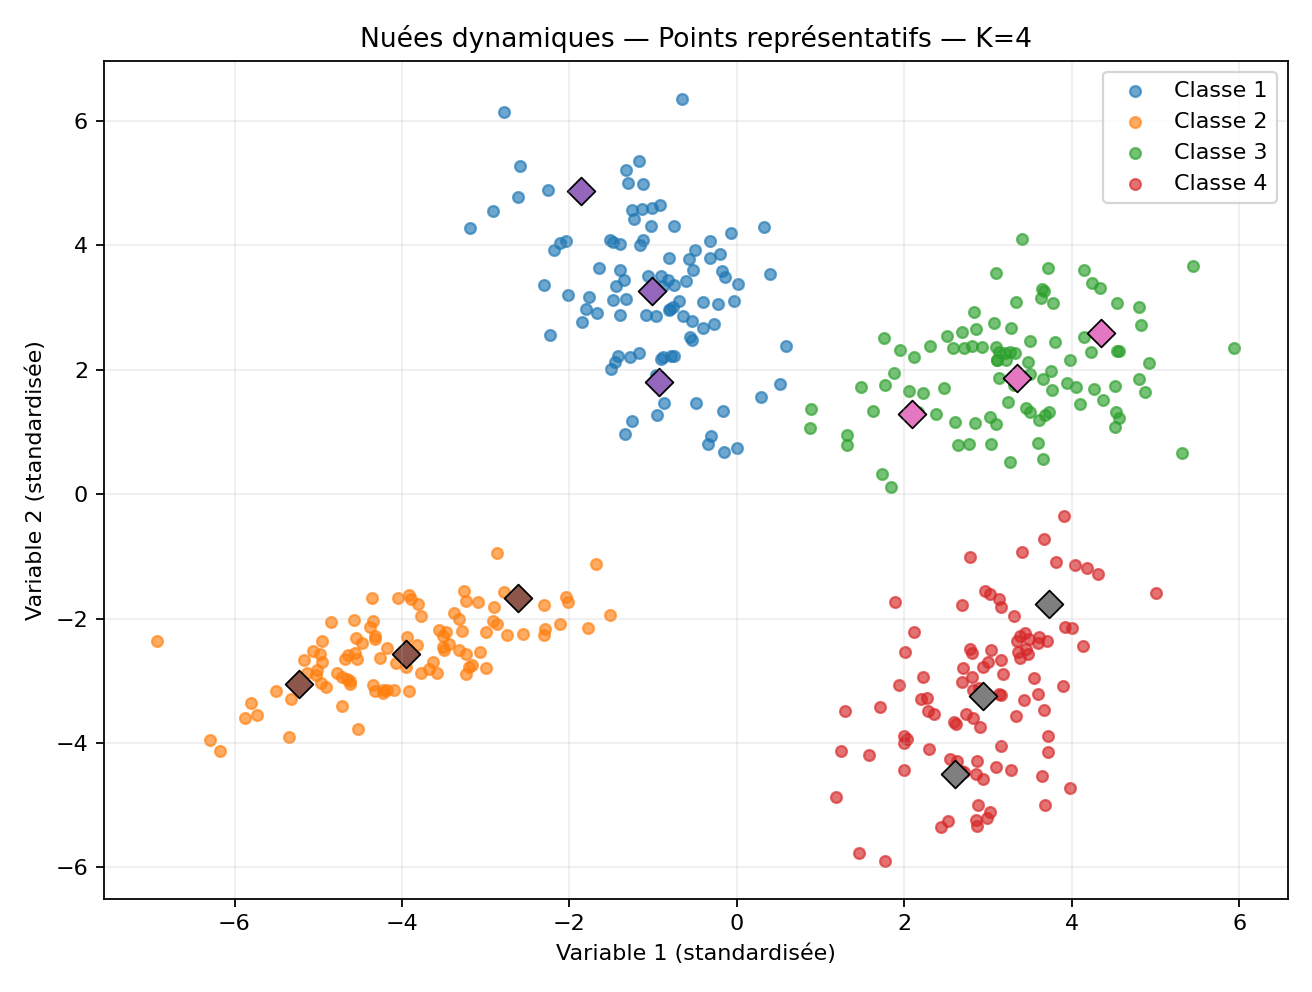
\includegraphics[width=0.82\textwidth]{../results/figures/points_partition.png}
\caption{Partition obtenue avec plusieurs points représentatifs par classe.}
\end{figure}

La figure permet d'observer les individus ainsi que les représentants utilisés pour caractériser chaque groupe.

\begin{figure}[H]
\centering
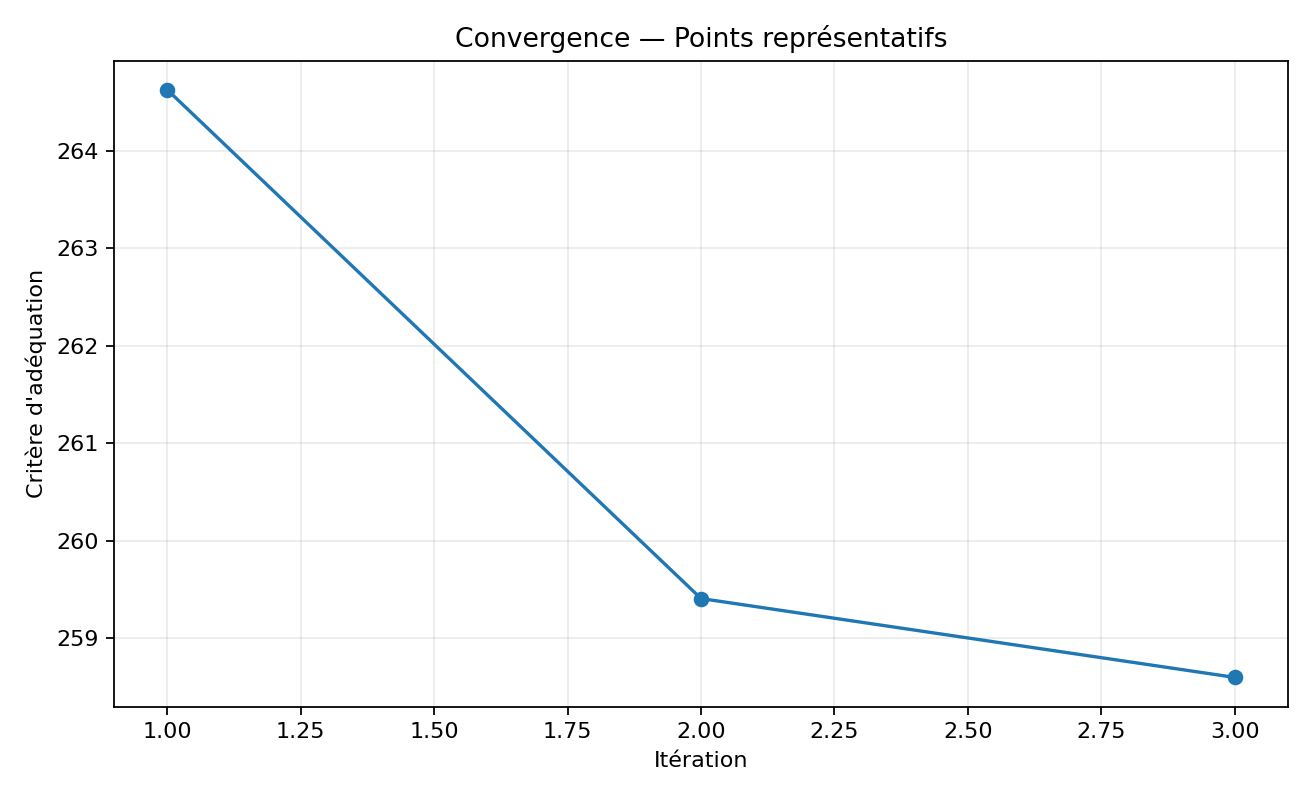
\includegraphics[width=0.78\textwidth]{../results/figures/points_convergence.png}
\caption{Évolution du critère pour la représentation par points.}
\end{figure}

\subsection{Axes factoriels}

\begin{figure}[H]
\centering
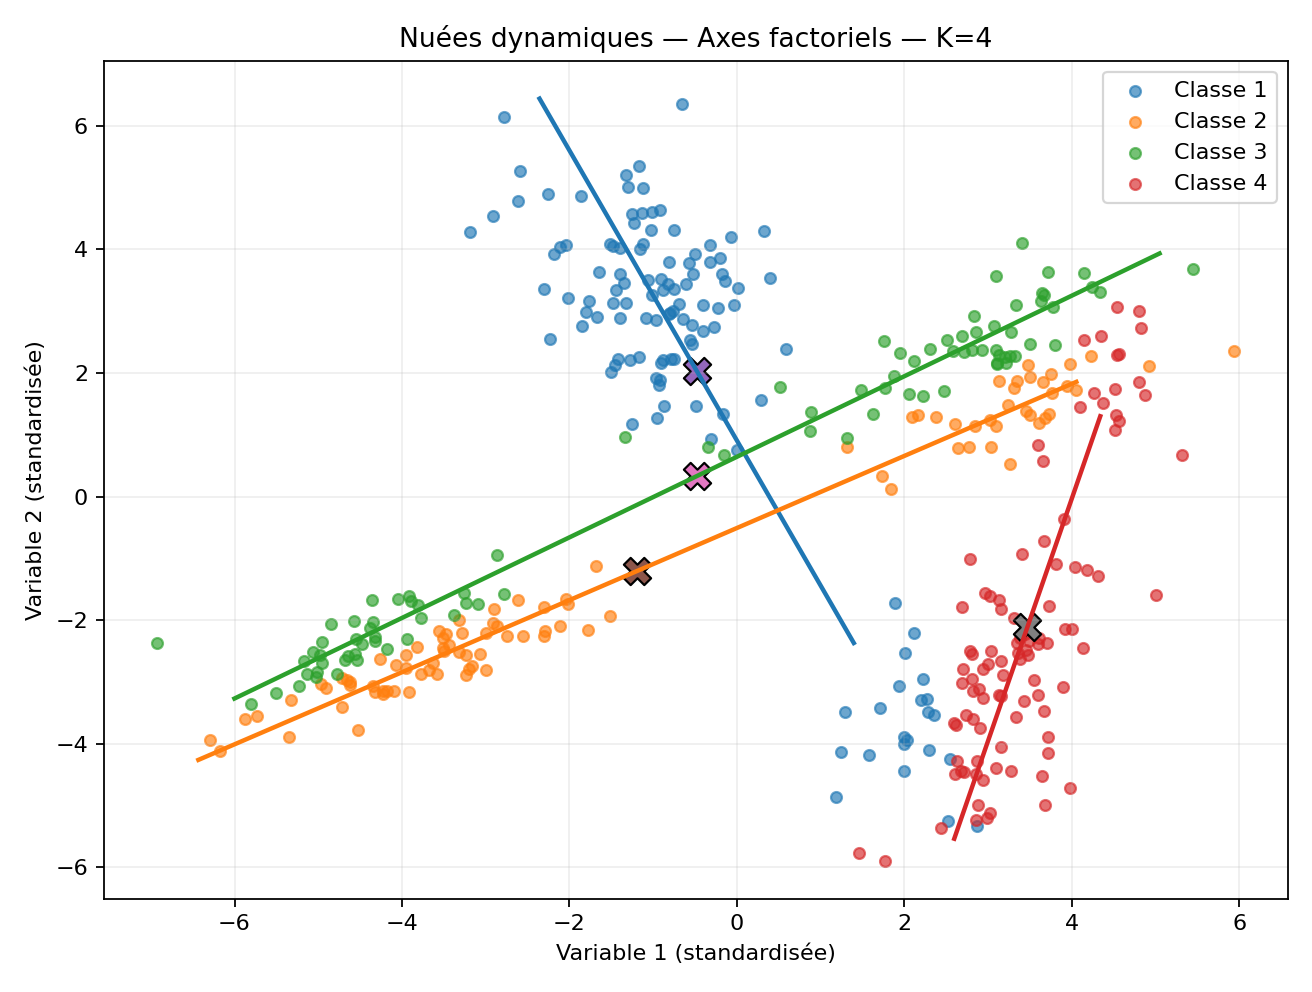
\includegraphics[width=0.82\textwidth]{../results/figures/axes_partition.png}
\caption{Partition et axes principaux des classes.}
\end{figure}

Ce mode cherche à conserver une structure directionnelle. Il est donc particulièrement intéressant lorsque la géométrie d'une classe n'est pas correctement résumée par un seul centre.

\begin{figure}[H]
\centering
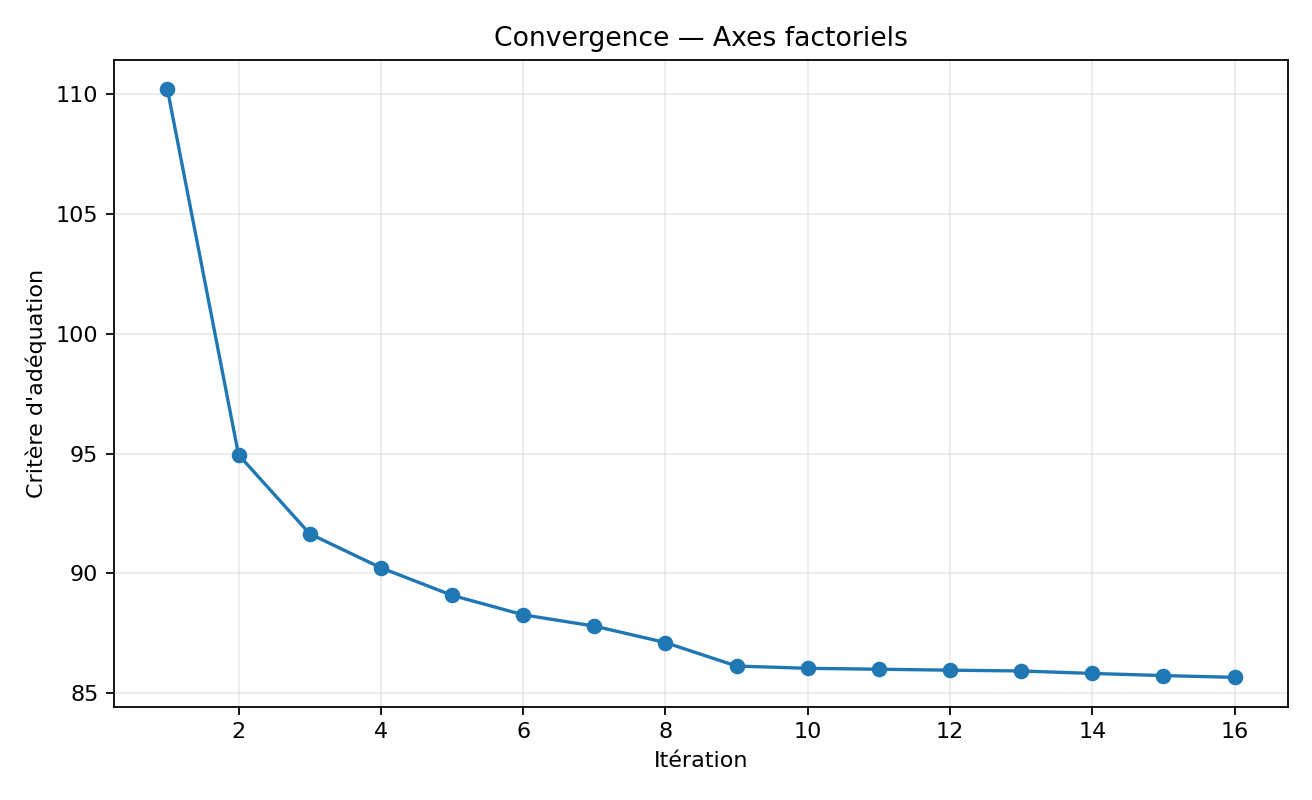
\includegraphics[width=0.78\textwidth]{../results/figures/axes_convergence.png}
\caption{Convergence de la représentation par axes.}
\end{figure}

\subsection{Distribution probabiliste}

\begin{figure}[H]
\centering
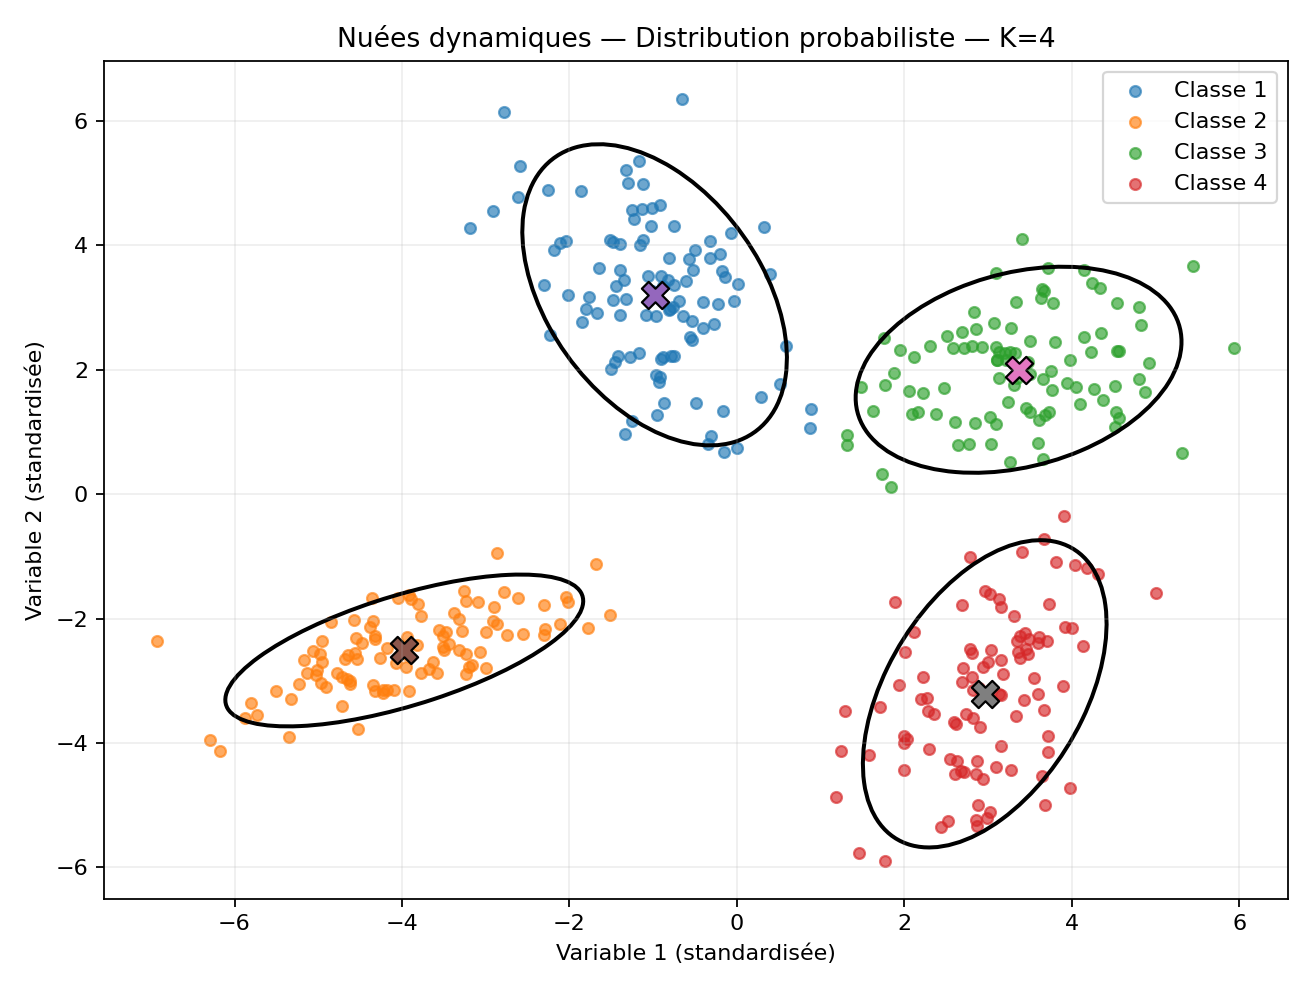
\includegraphics[width=0.82\textwidth]{../results/figures/distribution_partition.png}
\caption{Partition avec une représentation moyenne-covariance. Les ellipses visualisent la dispersion.}
\end{figure}

\begin{figure}[H]
\centering
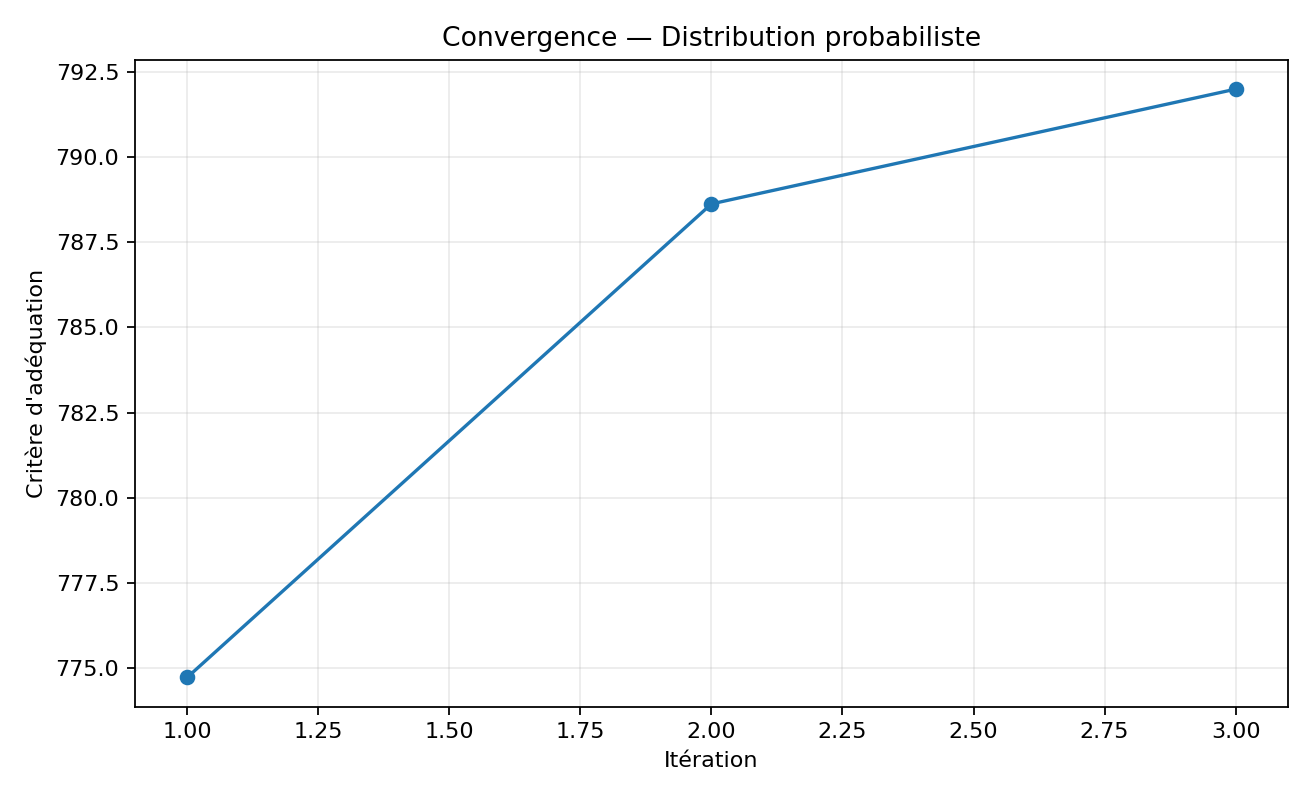
\includegraphics[width=0.78\textwidth]{../results/figures/distribution_convergence.png}
\caption{Convergence de la représentation probabiliste.}
\end{figure}

\subsection{Structure représentative}

\begin{figure}[H]
\centering
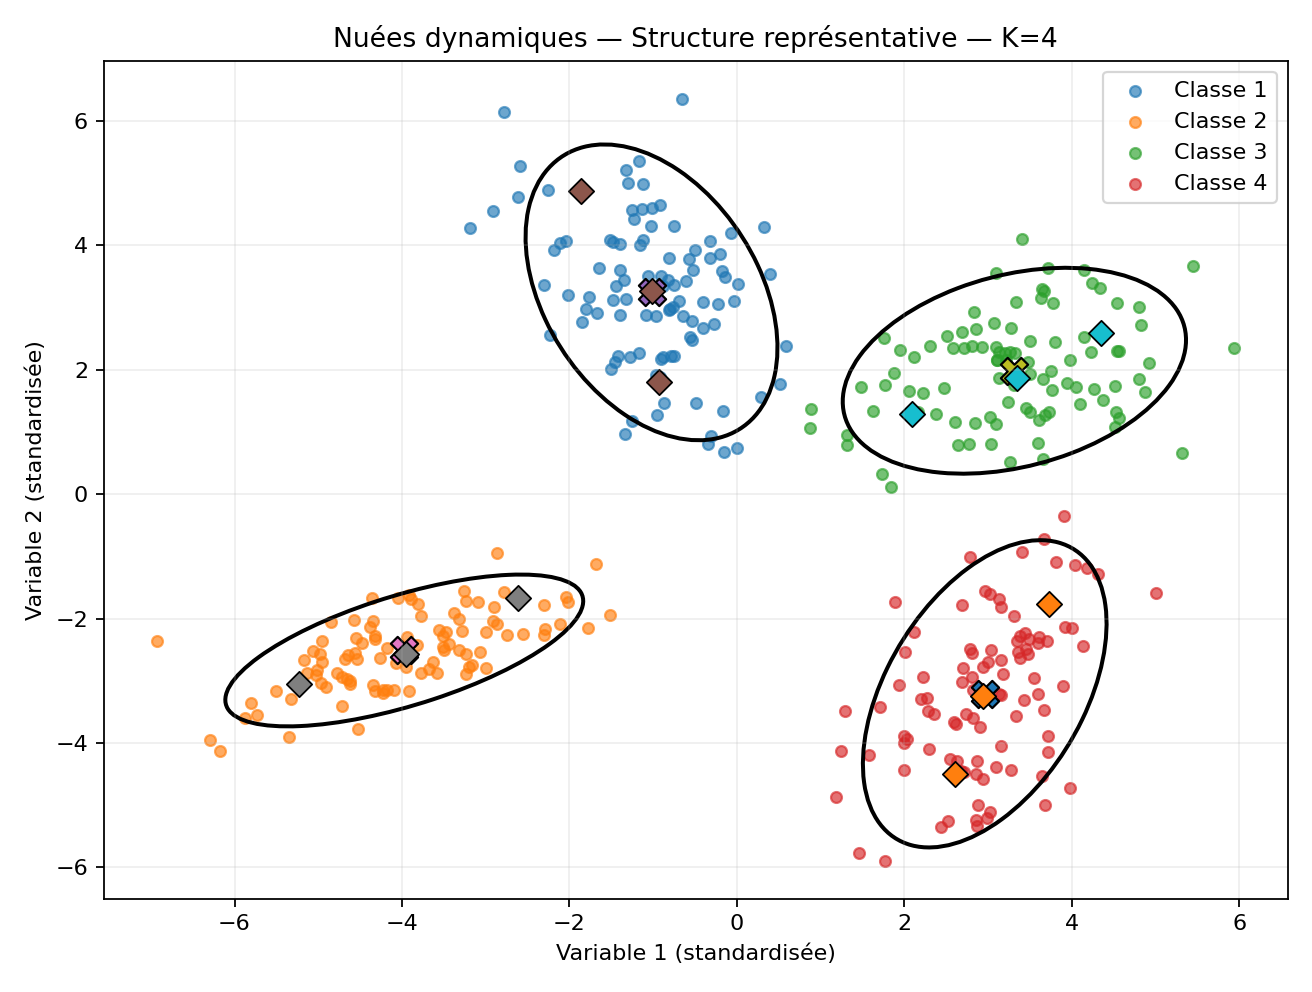
\includegraphics[width=0.82\textwidth]{../results/figures/structure_partition.png}
\caption{Structure représentative : centre, dispersion et étalons.}
\end{figure}

\begin{figure}[H]
\centering
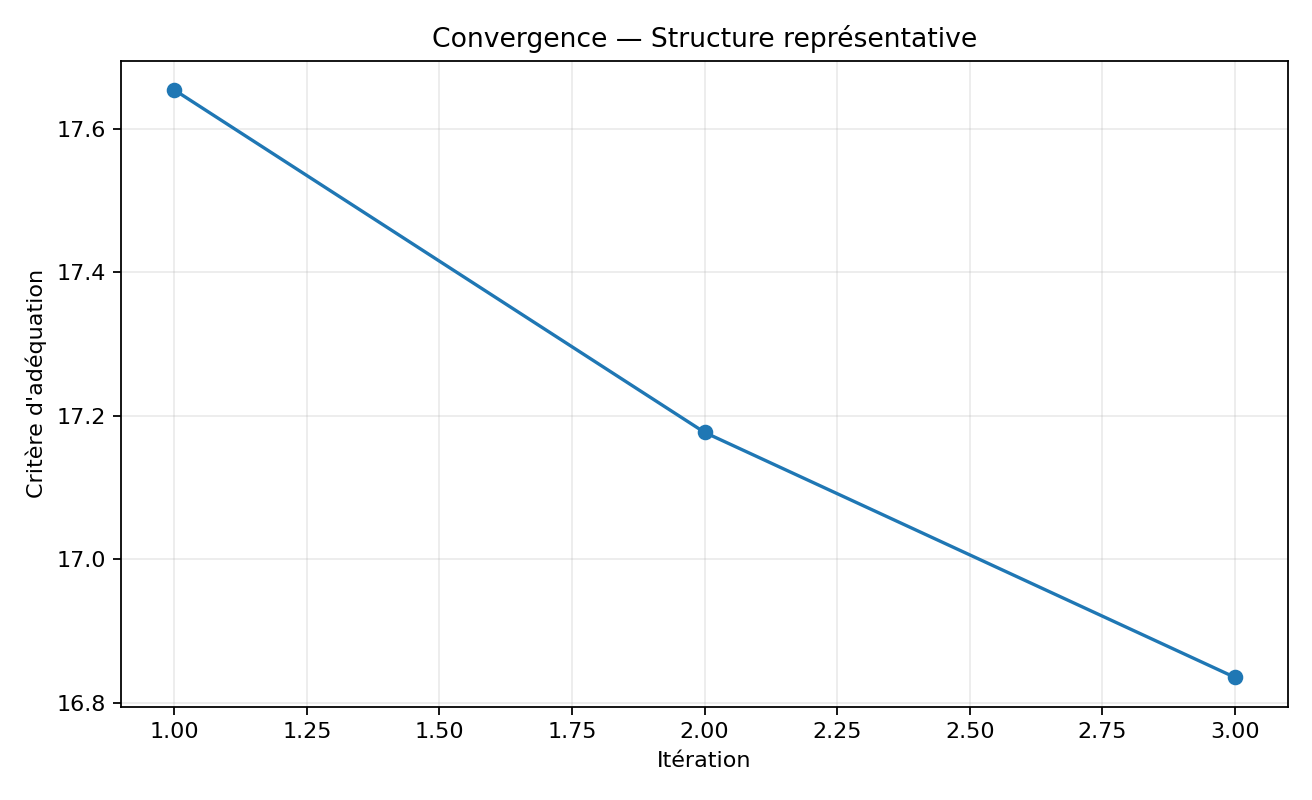
\includegraphics[width=0.78\textwidth]{../results/figures/structure_convergence.png}
\caption{Convergence de la structure représentative.}
\end{figure}

\subsection{Cas point : K-means}

\begin{figure}[H]
\centering
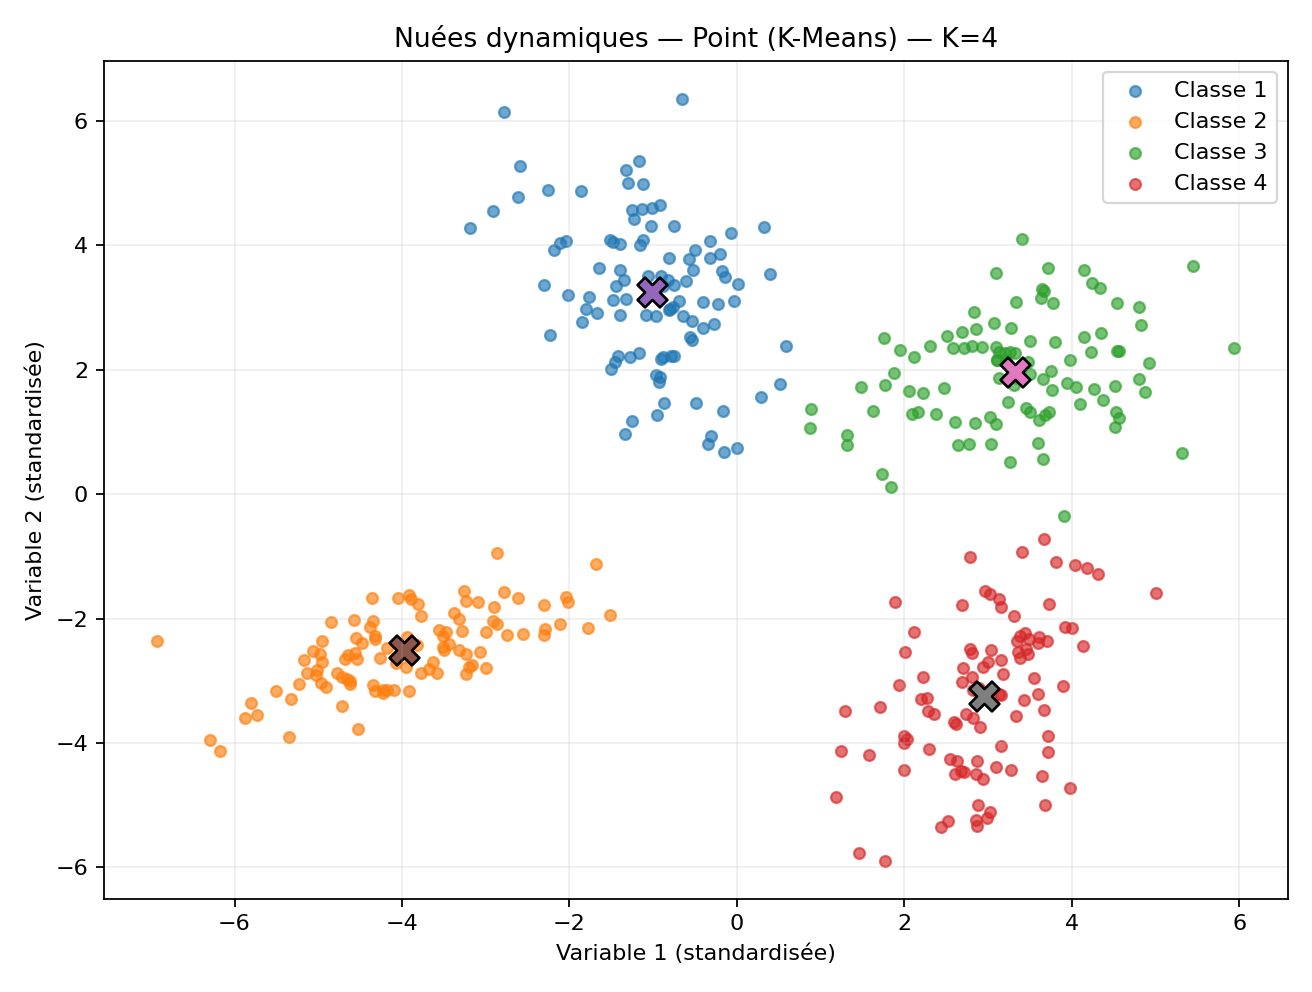
\includegraphics[width=0.82\textwidth]{../results/figures/point_partition.png}
\caption{Cas où chaque classe est représentée par un seul point.}
\end{figure}

\begin{figure}[H]
\centering
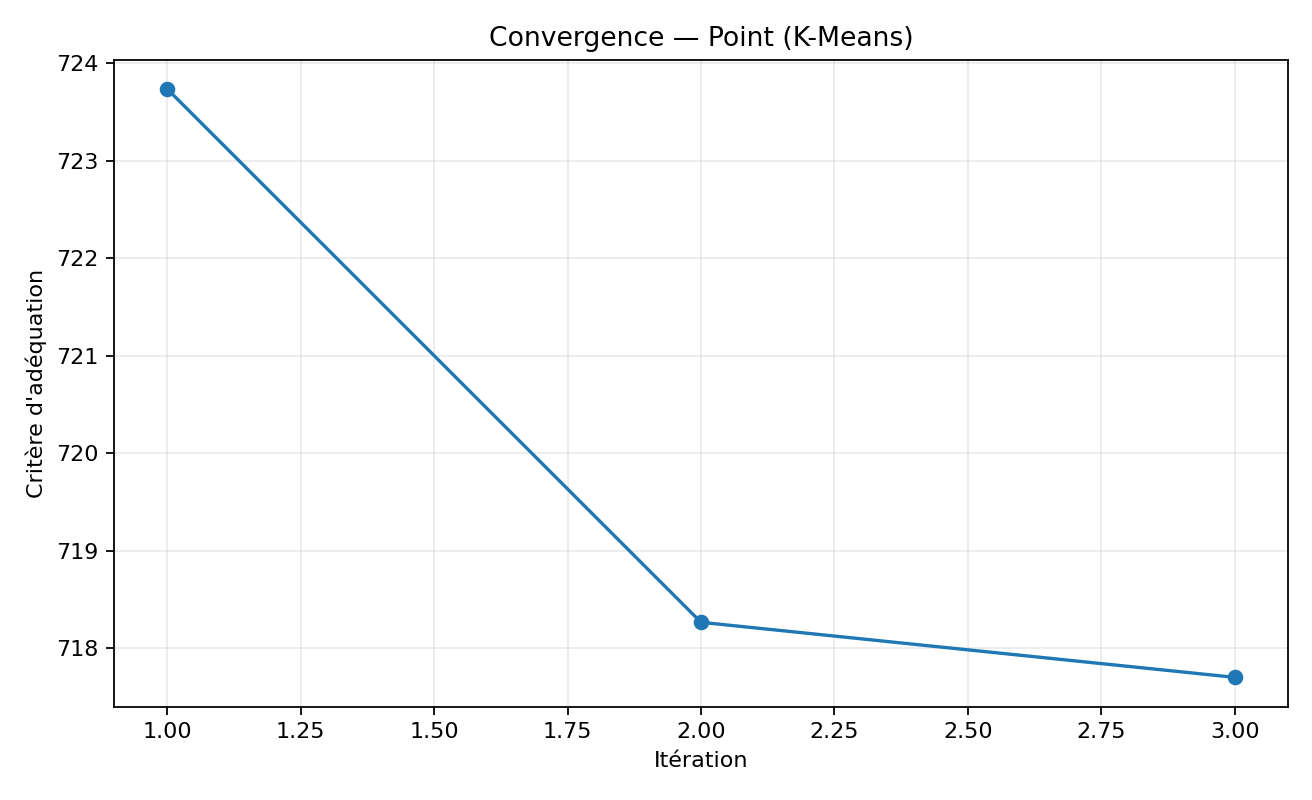
\includegraphics[width=0.78\textwidth]{../results/figures/point_convergence.png}
\caption{Convergence du cas K-means.}
\end{figure}

% =====================================================
\section{Analyse et discussion}
% =====================================================

\subsection{Influence de la représentation}

Le principal intérêt de l'application est de montrer qu'une même partition peut être abordée à partir de prototypes de nature différente. Un point résume essentiellement la position moyenne. Plusieurs étalons apportent une information spatiale plus riche. Les axes apportent une information directionnelle, tandis que la covariance introduit une information sur la dispersion et les corrélations.

Cette distinction est cohérente avec l'idée développée par Diday dans l'exemple artificiel de l'article : l'auteur observe que plusieurs étalons peuvent former un squelette de la forme et que le seul centre de gravité peut perdre l'information correspondant à des formes allongées \cite[p.~25]{diday1971}.

\subsection{Influence de l'initialisation}

Comme toute méthode itérative de partitionnement de ce type, l'initialisation peut influencer le résultat final. L'article de Diday insiste d'ailleurs sur l'intérêt d'effectuer plusieurs tirages de départ : lorsque des groupes similaires apparaissent de manière répétée, on peut obtenir une information sur la classifiabilité des données \cite[p.~24]{diday1971}.

Le programme utilise une graine afin de rendre l'expérience reproductible. Pour étudier l'influence de l'initialisation, il suffit de modifier `--seed`.

Exemple :

\begin{verbatim}
python main.py --mode points --k 4 --q 3 --seed 7
python main.py --mode points --k 4 --q 3 --seed 21
python main.py --mode points --k 4 --q 3 --seed 42
\end{verbatim}

Une extension naturelle du TP serait de répéter automatiquement l'algorithme plusieurs fois et de comparer les partitions obtenues.

\subsection{Classes vides}

Une classe peut devenir vide après une affectation. L'article original signale également l'apparition de classes vides lorsque le nombre de classes demandé est trop grand par rapport au nombre de groupes réellement présents \cite[p.~25]{diday1971}.

Dans notre implémentation, une classe vide est réparée en réaffectant à cette classe un individu provenant d'une classe non singleton. Cette stratégie permet au moteur de poursuivre l'itération sans abandonner l'expérience.

\subsection{Limites}

Les principales limites de cette implémentation sont :
\begin{itemize}
    \item les fonctions de distance sont volontairement simples ;
    \item la représentation probabiliste suppose une structure moyenne-covariance ;
    \item la structure représentative est une définition opérationnelle construite pour le TP ;
    \item l'algorithme n'explore pas automatiquement toutes les valeurs possibles de $K$ ;
    \item l'évaluation n'utilise pas ici de vérité terrain externe ;
    \item la visualisation est directement adaptée aux deux premières variables pour les données de dimension supérieure.
\end{itemize}

Ces limites ne remettent pas en cause l'objectif pédagogique principal : construire un moteur de classification dynamique dans lequel la nature du prototype peut être modifiée.

% =====================================================
\section{Tests et reproductibilité}
% =====================================================

Deux tests automatisés sont fournis. Ils vérifient :
\begin{enumerate}
    \item que les cinq représentations peuvent être entraînées sur le jeu de données de démonstration ;
    \item que le cas point construit bien un prototype par classe et permet la prédiction.
\end{enumerate}

La commande est :

\begin{verbatim}
python -m unittest discover -s tests -v
\end{verbatim}

Lors de la préparation du dépôt, les tests ont donné :

\begin{verbatim}
Ran 2 tests
OK
\end{verbatim}

La reproductibilité est obtenue en fixant 	exttt{seed=42} dans les expériences de référence.

% =====================================================
\section{Utilisation du projet}
% =====================================================

Le dépôt contient un script 	exttt{setup\_environment.py}. Contrairement à un simple appel systématique à 	exttt{pip install -r requirements.txt}, ce script vérifie d'abord la présence et la version des bibliothèques nécessaires. Si elles sont déjà satisfaisantes, aucun téléchargement n'est effectué.

Pour lancer le projet :

\begin{verbatim}
python setup_environment.py
python main.py
\end{verbatim}

Ou, directement sous Windows :

\begin{verbatim}
run_windows.bat
\end{verbatim}

Le fichier `README.md` contient toutes les commandes détaillées ainsi que la procédure pour utiliser un autre fichier CSV et publier le projet sur GitHub.

% =====================================================
\section{Conclusion}
% =====================================================

Ce travail a permis de réaliser une implémentation from scratch du principe des Nuées dynamiques en construisant un moteur générique capable de fonctionner avec plusieurs représentations de classes.

Le point essentiel est l'alternance entre l'affectation des individus et la reconstruction des représentations. Dans le cas le plus simple, la représentation est réduite à un point et l'on retrouve le principe du K-means. En revanche, l'utilisation de plusieurs étalons, d'axes, d'une covariance ou d'une structure composite permet de conserver davantage d'information sur la forme d'une classe.

Le travail est directement inspiré de la formulation de Diday : l'article de 1971 définit le problème de partitionnement, formalise les configurations, décrit l'algorithme itératif et étudie la convergence. Il met également en évidence l'intérêt des étalons pour représenter des formes qui seraient trop grossièrement résumées par un seul centre \cite{diday1971}.

L'application réalisée constitue donc une base pédagogique permettant d'expérimenter concrètement l'idée centrale du TP : \textbf{la Nuée dynamique fournit un cadre général dans lequel la représentation d'une classe peut être adaptée au problème étudié.}

% =====================================================
\begin{thebibliography}{9}

\bibitem{diday1971}
E. Diday,
\textit{Une nouvelle méthode en classification automatique et reconnaissance des formes : la méthode des nuées dynamiques},
Revue de Statistique Appliquée, tome 19, n° 2, 1971, pp. 19--33.
Disponible sur NumDAM :
\url{https://www.numdam.org/item/RSA_1971__19_2_19_0/}.

\end{thebibliography}

\end{document}
